\documentclass[11pt]{article}

\usepackage[margin=1in]{geometry}
\usepackage[T1]{fontenc}
\usepackage[utf8]{inputenc}
\usepackage{amsmath,amssymb,amsthm}
\usepackage{booktabs}
\usepackage{graphicx}
\usepackage{array}
\usepackage{caption}
\usepackage[numbers]{natbib}
\usepackage[colorlinks=true,allcolors=blue]{hyperref}

\graphicspath{{../figures/}}

\newtheorem{proposition}{Proposition}

\title{Median-Length Exact-Coverage Confidence Intervals for the Power of the One-Sample t-Test}
\author{Harrison Watts}
\date{April 2026}

\begin{document}

\maketitle

\begin{abstract}
Tarasi\'{n}ska's interval for the power of the one-sample Student t-test is built by transforming a confidence interval for the unknown standard deviation, while Chakraborti, Michaelson, and McCracken later repaired the coverage problem of the minimum-length version by minimizing expected interval length over the randomness of the sample standard deviation. This note studies the corresponding median-length criterion, interpreted pointwise at a prespecified standardized shift $\kappa=\Delta/\sigma$ fixed at the design stage. The resulting construction preserves exact coverage because the chi-squared pivot endpoints are fixed before observing the data, but it replaces the expected-length objective with the median of the random interval length and computes the allocation numerically. The primary computation uses a deterministic chi-squared quantile grid; a Monte Carlo approximation to the same length distribution is included as a computational sensitivity analysis rather than as a separate inferential construction. Across a grid of sample sizes and standardized shifts, the deterministically computed median-length interval achieves its largest additional median-length improvement over the expected-length interval at $0.62\%$ on the study grid, while the Monte Carlo approximation closely tracks the same allocations and length gains. The broader comparison shows that mean and median interval widths can differ sharply in finite samples. Full-grid Monte Carlo validation confirms agreement with the nominal $95\%$ coverage throughout, as expected from the exact-coverage construction, and serves as a check of the numerical implementation rather than empirical corroboration of the theoretical result. The median criterion is best viewed as a calibrated interpretive complement to the expected-length benchmark rather than a wholesale replacement.
\end{abstract}

\section{Introduction}
The power of Student's one-sample t-test depends on the unknown population standard deviation, so any post-data assessment of power inherits uncertainty from estimating $\sigma$. Tarasi\'{n}ska \citep{tarasinska2005power} proposed a confidence interval for the power of the one-sided test by transforming a chi-squared confidence interval for $\sigma$. Gilliland and Li \citep{gilliland2008note} later showed that Tarasi\'{n}ska's minimum-length implementation does not attain the advertised nominal coverage because its interval endpoints depend on the observed sample standard deviation. Chakraborti, Michaelson, and McCracken \citep{chakraborti2012shortest} addressed that issue by choosing the chi-squared endpoints in advance and minimizing the \emph{expected} length of the resulting random power interval.

The next natural step in that sequence is to replace the expected-length criterion with a \emph{median}-length criterion. That objective is attractive when the random interval length is highly asymmetric, since a mean can be heavily influenced by a relatively small set of long intervals. At the same time, modern statistical practice cautions against using post hoc power as a substitute for effect-size estimation or interval estimation \citep{hoenig2001abuse,greenland2016misinterpretations}. The present note therefore keeps the methodological target narrow: it studies the power function indexed by a prespecified standardized shift $\kappa=\Delta/\sigma$, treated as a design-stage quantity rather than estimated from the observed data. Under this interpretation, the paper does not claim exact post-data inference for a raw effect $\Delta$ with unknown standardization. Instead, it studies interval procedures whose exact-coverage statement holds pointwise for each fixed $\kappa$. Exact coverage fails if $\kappa$ or the allocation $p$ is chosen post hoc from the data.

This note makes three contributions. First, it rewrites the power-interval construction in a scale-free form indexed by the standardized shift $\kappa=\Delta/\sigma$. Second, it defines the population median-length exact-coverage criterion and computes a deterministic numerical approximation to its optimizer. Third, it runs a reproducible numerical study that compares the resulting intervals with equal-tail and expected-length competitors on both mean and median length, uses a Monte Carlo approximation to the median objective as a computational sensitivity analysis, and validates coverage by Monte Carlo simulation across the full design grid. An important part of the empirical message is comparative rather than triumphant: even when the length distribution is skewed enough for mean and median width to differ materially, the classical expected-length rule is often already close to the median-length benchmark. In that sense, the paper is intended not only as a new criterion study but also as an exact finite-sample benchmark for a class of ``robust width'' questions.

\section{Exact-Coverage Power Intervals}
Let $X_1,\dots,X_n$ be independent and identically distributed as $N(\mu,\sigma^2)$. We test
\[
H_0:\mu=\mu_0 \qquad \text{versus} \qquad H_1:\mu>\mu_0
\]
with the usual one-sample t statistic
\[
T = \frac{\sqrt{n}(\bar X-\mu_0)}{S},
\qquad
S^2=\frac{1}{n-1}\sum_{i=1}^{n}(X_i-\bar X)^2,
\]
and reject for $T>t_{1-\alpha,\nu}$, where $\nu=n-1$.

If the true mean satisfies $\mu=\mu_0+\Delta$ with $\Delta>0$, then the power can be written as
\[
\pi_{n,\alpha}(\kappa)
=
1-G_{\nu,\sqrt{n}\kappa}\!\left(t_{1-\alpha,\nu}\right),
\qquad
\kappa=\frac{\Delta}{\sigma},
\]
where $G_{\nu,\delta}$ is the cumulative distribution function of the noncentral t distribution with $\nu$ degrees of freedom and noncentrality parameter $\delta$ \citep{tarasinska2005power}. Thus the power is determined by the standardized shift $\kappa$.

Now define the pivotal quantity
\[
Q=\frac{\nu S^2}{\sigma^2}\sim \chi^2_{\nu}.
\]
For constants $0\leq A<B$ satisfying
\[
\Pr(A\leq Q\leq B)=1-\gamma,
\]
the induced confidence interval for $\sigma$ is
\[
\left[\sqrt{\frac{\nu S^2}{B}},\sqrt{\frac{\nu S^2}{A}}\right].
\]
Because $\pi_{n,\alpha}(\kappa)$ is decreasing in $\sigma$ for fixed $\Delta$, the corresponding interval for power is
\[
C_{A,B}(Q)
=
\left[
\pi_{n,\alpha}\!\left(\kappa\sqrt{\frac{A}{Q}}\right),
\pi_{n,\alpha}\!\left(\kappa\sqrt{\frac{B}{Q}}\right)
\right].
\]

\begin{proposition}
For constants $A$ and $B$ chosen before observing $S$, with $\Pr(A\le Q\le B)=1-\gamma$, the interval $C_{A,B}(Q)$ has exact coverage:
\[
\Pr\!\left\{\pi_{n,\alpha}(\kappa)\in C_{A,B}(Q)\right\}=1-\gamma.
\]
\end{proposition}

\begin{proof}
The map $\sigma \mapsto \pi_{n,\alpha}(\Delta/\sigma)$ is monotone decreasing. Therefore
\[
\pi_{n,\alpha}(\kappa)\in C_{A,B}(Q)
\iff
\sqrt{\frac{\nu S^2}{B}}\le \sigma \le \sqrt{\frac{\nu S^2}{A}}
\iff
A\le Q\le B.
\]
Taking probabilities yields $1-\gamma$.
\end{proof}

\noindent\textit{Remark.} The monotone transformation through $\sigma$ is a construction device; the resulting coverage statement is pointwise in the fixed index~$\kappa$. Exact coverage therefore holds for each prespecified standardized alternative~$\kappa$. It does not automatically hold if $\kappa$, or equivalently the allocation~$p$, is estimated or selected from the observed data, because $A$ and $B$ would then depend on $S$ and the chain of equivalences in the proof would no longer go through exactly. Practitioners who wish to use this interval should fix $\kappa$ at the design stage and not revise it in light of the observed sample standard deviation.

\noindent Following Chakraborti et al.\ \citep{chakraborti2012shortest}, it is convenient to parameterize admissible intervals by the left-tail probability
\[
p=\Pr(Q<A), \qquad 0\le p\le \gamma,
\]
so that
\[
A_p = F_{\chi^2_\nu}^{-1}(p),
\qquad
B_p = F_{\chi^2_\nu}^{-1}(p+1-\gamma).
\]
The random interval length becomes
\[
\Lambda_p(Q;\kappa)
=
\pi_{n,\alpha}\!\left(\kappa\sqrt{\frac{B_p}{Q}}\right)
-
\pi_{n,\alpha}\!\left(\kappa\sqrt{\frac{A_p}{Q}}\right).
\]
This expression depends on the problem only through $(n,\alpha,\gamma,\kappa)$, so the resulting tables are scale free.

The admissible range $0\le p\le\gamma$ has natural boundary interpretations. At $p=0$, $A_0=0$, giving a chi-squared interval for $\sigma$ with no finite lower bound and a one-sided lower power interval. At $p=\gamma$, $B_\gamma = F_{\chi^2_\nu}^{-1}(1)=\infty$, giving a power interval of the form $[\pi_{n,\alpha}(\kappa\sqrt{A_\gamma/Q}),\,1]$ with the upper endpoint fixed at~1. Because $B_\gamma$ is not a finite real number, the numerical search below is conducted over a compact subinterval of $(0,\gamma)$ with small tolerances at each boundary, and the limiting one-sided constructions at the endpoints are understood as excluded limits.

\section{Expected and Median Length Criteria}
The main comparison concerns three exact-coverage interval constructions, together with one Monte Carlo approximation to the median-length optimizer used as a numerical sensitivity analysis.

\begin{enumerate}
\item \textbf{Equal-tail}: $p=\gamma/2$.
\item \textbf{Expected-opt}: define the population target
\[
\quad
p_E^\star \in \arg\min_{0\le p\le \gamma} E\{\Lambda_p(Q;\kappa)\},
\]
which reproduces the criterion of \citet{chakraborti2012shortest}.
\item \textbf{Median-opt}: define the population target
\[
\quad
p_M^\star \in \arg\min_{0\le p\le \gamma} \operatorname{Med}\{\Lambda_p(Q;\kappa)\},
\]
which is the proposed median-length analogue.
\item \textbf{Median-MC}: draw $Q_1,\dots,Q_R \stackrel{\mathrm{iid}}{\sim}\chi^2_\nu$ once at the design stage and define the simulation-based approximation
\[
\quad
\widehat p_{M,R}^{\,MC} \in \arg\min_{0\le p\le \gamma} \operatorname{Med}\{\Lambda_p(Q_1;\kappa),\dots,\Lambda_p(Q_R;\kappa)\},
\]
which approximates the same median-length target by simulation.
\end{enumerate}

The median criterion does not alter the exact-coverage argument because it changes only the \emph{design-stage} choice of $A_p$ and $B_p$, not the pivotal construction itself. What it changes is the notion of optimality. The expected-length interval is natural under an average-loss objective. The median-length interval instead targets the typical realized width, which can be more interpretable when the distribution of $\Lambda_p(Q;\kappa)$ is far from symmetric. In the numerical work below, the reported quantities labeled $p_E$ and $p_M$ are computed approximations to the population targets $p_E^\star$ and $p_M^\star$, obtained by bounded one-dimensional search on deterministic objective evaluations. Likewise, the reported quantity labeled $p_{MC}$ is the computed Monte Carlo approximation $\widehat p_{M,R}^{\,MC}$ for a fixed simulated sample. Thus ``Expected-opt,'' ``Median-opt,'' and ``Median-MC'' should be read as numerically implemented procedures rather than as claims of closed-form analytic solutions or exact numerical minimization.

\section{Numerical Study}
\subsection{Design}
All computations use $\alpha=\gamma=0.05$. The grid of sample sizes is
\[
n\in\{2,4,8,16,25\},
\]
and the grid of standardized shifts is
\[
\kappa\in\{0.25,0.50,0.75,1.00,1.25\}.
\]
For each $(n,\kappa)$ pair, the deterministic objective functions were evaluated on a grid of 4{,}001 midpoint chi-squared quantiles and optimized over a compact subinterval of $(0,\gamma)$ by one-dimensional bounded search with absolute tolerance $10^{-6}$ on $p$. The simulation-based median approximation used a fixed common-random-numbers sample of size $R=4{,}000$ from $\chi^2_\nu$ for each $n$, with the sample held fixed during the optimization so that the objective remained reproducible across candidate allocations. Because the sample median objective is nonsmooth and can be locally flat, the resulting Monte Carlo optimizer should be interpreted as a sensitivity analysis for the deterministic solution rather than as an independent optimality theory. Because the interval depends on the data only through $Q$, the Monte Carlo validation simulates $Q\sim\chi^2_\nu$ directly rather than regenerating the full normal sample each time. The script \texttt{scripts/median\_power\_ci.py} reproduces every table and figure in the paper.

\subsection{Main results}
Classical statistical writing often reports the full design grid, and that format is also useful here because the boundary behavior of the optimization is itself part of the numerical story. Accordingly, Tables~\ref{tab:optima} and \ref{tab:lengths} display the complete $25$-point grid for the principal summaries.

\begin{table}[htbp]
\centering
\caption{Computed tail allocations, reported as $p_E$, $p_M$, and $p_{MC}$ for compactness, together with summary diagnostics for the expected-length interval, the deterministic median-length interval, and the Monte Carlo median-length sensitivity analysis over the full design grid.}
\label{tab:optima}
\resizebox{\textwidth}{!}{\begin{tabular}{ccrrrrrr}
\toprule
$n$ & $\kappa$ & $p_E$ & $p_M$ & $p_{MC}$ & Mean/Median$_E$ & Med gain M (\%) & Med gain MC (\%) \\
\midrule
2 & 0.25 & 0.0000 & 0.0000 & 0.0001 & 2.197 & 0.00 & -0.03 \\
2 & 0.50 & 0.0000 & 0.0000 & 0.0001 & 1.581 & 0.00 & -0.03 \\
2 & 0.75 & 0.0000 & 0.0000 & 0.0002 & 1.311 & 0.00 & -0.09 \\
2 & 1.00 & 0.0000 & 0.0000 & 0.0001 & 1.162 & 0.00 & -0.04 \\
2 & 1.25 & 0.0006 & 0.0003 & 0.0001 & 1.067 & 0.10 & 0.11 \\
\midrule
4 & 0.25 & 0.0049 & 0.0046 & 0.0046 & 1.427 & 0.00 & 0.00 \\
4 & 0.50 & 0.0068 & 0.0031 & 0.0032 & 1.164 & 0.42 & 0.42 \\
4 & 0.75 & 0.0135 & 0.0066 & 0.0062 & 0.978 & 0.62 & 0.62 \\
4 & 1.00 & 0.0263 & 0.0268 & 0.0267 & 0.933 & 0.00 & 0.00 \\
4 & 1.25 & 0.0401 & 0.0374 & 0.0355 & 0.932 & 0.07 & 0.04 \\
\midrule
8 & 0.25 & 0.0104 & 0.0099 & 0.0099 & 1.156 & 0.00 & 0.00 \\
8 & 0.50 & 0.0168 & 0.0120 & 0.0129 & 1.001 & 0.24 & 0.23 \\
8 & 0.75 & 0.0347 & 0.0326 & 0.0302 & 0.949 & 0.04 & -0.03 \\
8 & 1.00 & 0.0480 & 0.0500 & 0.0499 & 0.920 & 0.60 & 0.59 \\
8 & 1.25 & 0.0499 & 0.0500 & 0.0499 & 0.948 & 0.04 & 0.00 \\
\midrule
16 & 0.25 & 0.0151 & 0.0144 & 0.0144 & 1.054 & 0.01 & 0.01 \\
16 & 0.50 & 0.0301 & 0.0297 & 0.0312 & 0.968 & 0.01 & -0.03 \\
16 & 0.75 & 0.0481 & 0.0498 & 0.0498 & 0.959 & 0.39 & 0.39 \\
16 & 1.00 & 0.0500 & 0.0500 & 0.0499 & 1.089 & 0.01 & -0.05 \\
16 & 1.25 & 0.0500 & 0.0500 & 0.0499 & 1.447 & 0.00 & -0.10 \\
\midrule
25 & 0.25 & 0.0184 & 0.0177 & 0.0177 & 1.019 & 0.01 & 0.01 \\
25 & 0.50 & 0.0392 & 0.0397 & 0.0397 & 0.944 & 0.00 & 0.00 \\
25 & 0.75 & 0.0498 & 0.0500 & 0.0499 & 1.073 & 0.10 & 0.06 \\
25 & 1.00 & 0.0500 & 0.0500 & 0.0499 & 1.541 & 0.00 & -0.09 \\
25 & 1.25 & 0.0500 & 0.0500 & 0.0499 & 3.324 & 0.00 & -0.14 \\
\bottomrule
\end{tabular}
}
\end{table}

Several patterns are worth highlighting. First, the deterministically computed median-length and expected-length allocations are often very close, and they coincide on the boundary for many settings. On the study grid, the largest additional median-length improvement of the deterministic median-length interval over the expected-length interval is only $0.62\%$, attained at $(n,\kappa)=(4,0.75)$. The Monte Carlo approximation tracks this pattern closely: its computed allocations generally remain near $p_M$, and its implied median-length gains are of the same small order. The few slightly negative Monte Carlo gains visible in Table~\ref{tab:optima} should be read as approximation error from the simulated objective, not as evidence against the deterministic criterion. Second, departures between the mean and median widths can nevertheless be large. The mean-to-median ratio ranges from $0.92$ to $3.32$, so an average-length criterion can substantially overstate or understate the typical realized width. Third, the repeated endpoint values in the upper-right part of Table~\ref{tab:optima} are not accidental duplication: they indicate that the numerical optimum lies at the upper boundary of the search region; within a fixed $n$, settings whose optimizer converges to this boundary share the same chi-squared endpoint pair because $A_p$ and $B_p$ are determined solely by $p$ and $\nu$, not by $\kappa$.

Table~\ref{tab:lengths} compares the actual mean and median lengths of the three principal procedures over the full design grid. The equal-tail interval is consistently dominated in the smaller-sample settings. The median-length interval yields the intended improvement in the median column, but the gain over the expected-length interval is modest, which suggests that Chakraborti et al.'s expected-length construction is already close to the median benchmark in many cases. That ``small-gain'' finding is itself useful: it shows that, for this classical problem, optimizing average width already gets one surprisingly close to optimizing typical width. The Monte Carlo analogue is omitted from this table both to keep the full-grid presentation readable and because its role here is diagnostic rather than primary; its performance is summarized in Table~\ref{tab:optima} and revisited in the validation table below.

\begin{table}[htbp]
\centering
\caption{Mean and median lengths for equal-tail (ET), expected-length (EO), and median-length (MO) exact-coverage intervals over the full design grid.}
\label{tab:lengths}
\resizebox{\textwidth}{!}{\begin{tabular}{ccrrrrrr}
\toprule
$n$ & $\kappa$ & Mean ET & Mean EO & Mean MO & Median ET & Median EO & Median MO \\
\midrule
2 & 0.25 & 0.2079 & 0.1925 & 0.1925 & 0.1020 & 0.0876 & 0.0876 \\
2 & 0.50 & 0.3416 & 0.3209 & 0.3209 & 0.2337 & 0.2030 & 0.2030 \\
2 & 0.75 & 0.4415 & 0.4200 & 0.4200 & 0.3616 & 0.3203 & 0.3203 \\
2 & 1.00 & 0.5192 & 0.4994 & 0.4994 & 0.4756 & 0.4297 & 0.4297 \\
2 & 1.25 & 0.5809 & 0.5643 & 0.5643 & 0.5732 & 0.5291 & 0.5286 \\
\midrule
4 & 0.25 & 0.1848 & 0.1744 & 0.1744 & 0.1310 & 0.1223 & 0.1223 \\
4 & 0.50 & 0.4223 & 0.4075 & 0.4088 & 0.3760 & 0.3500 & 0.3485 \\
4 & 0.75 & 0.5958 & 0.5900 & 0.5930 & 0.6192 & 0.6035 & 0.5998 \\
4 & 1.00 & 0.6916 & 0.6916 & 0.6916 & 0.7414 & 0.7412 & 0.7412 \\
4 & 1.25 & 0.7292 & 0.7180 & 0.7185 & 0.7775 & 0.7704 & 0.7699 \\
\midrule
8 & 0.25 & 0.1961 & 0.1900 & 0.1900 & 0.1703 & 0.1644 & 0.1644 \\
8 & 0.50 & 0.4792 & 0.4758 & 0.4771 & 0.4828 & 0.4754 & 0.4742 \\
8 & 0.75 & 0.5953 & 0.5904 & 0.5907 & 0.6256 & 0.6224 & 0.6221 \\
8 & 1.00 & 0.5590 & 0.5189 & 0.5250 & 0.6109 & 0.5642 & 0.5607 \\
8 & 1.25 & 0.4612 & 0.3928 & 0.3929 & 0.4993 & 0.4142 & 0.4140 \\
\midrule
16 & 0.25 & 0.2292 & 0.2261 & 0.2261 & 0.2180 & 0.2145 & 0.2145 \\
16 & 0.50 & 0.4611 & 0.4598 & 0.4598 & 0.4764 & 0.4753 & 0.4752 \\
16 & 0.75 & 0.3677 & 0.3344 & 0.3363 & 0.3920 & 0.3486 & 0.3472 \\
16 & 1.00 & 0.1964 & 0.1551 & 0.1551 & 0.1902 & 0.1424 & 0.1424 \\
16 & 1.25 & 0.0843 & 0.0584 & 0.0584 & 0.0662 & 0.0404 & 0.0404 \\
\midrule
25 & 0.25 & 0.2536 & 0.2521 & 0.2521 & 0.2493 & 0.2475 & 0.2474 \\
25 & 0.50 & 0.3625 & 0.3533 & 0.3533 & 0.3832 & 0.3741 & 0.3741 \\
25 & 0.75 & 0.1596 & 0.1319 & 0.1321 & 0.1551 & 0.1230 & 0.1228 \\
25 & 1.00 & 0.0402 & 0.0279 & 0.0279 & 0.0291 & 0.0181 & 0.0181 \\
25 & 1.25 & 0.0071 & 0.0041 & 0.0041 & 0.0027 & 0.0012 & 0.0012 \\
\bottomrule
\end{tabular}
}
\end{table}

Figure~\ref{fig:lengths} shows the full distribution of interval lengths in two representative cases. For $n=2$ and $\kappa=0.50$, the random length is highly dispersed and the mean exceeds the median under all three procedures. By $n=8$, the competing optimized intervals are much closer, which explains why the full tables show only incremental gains of the median-length criterion over the expected-length benchmark.

\begin{figure}[htbp]
\centering
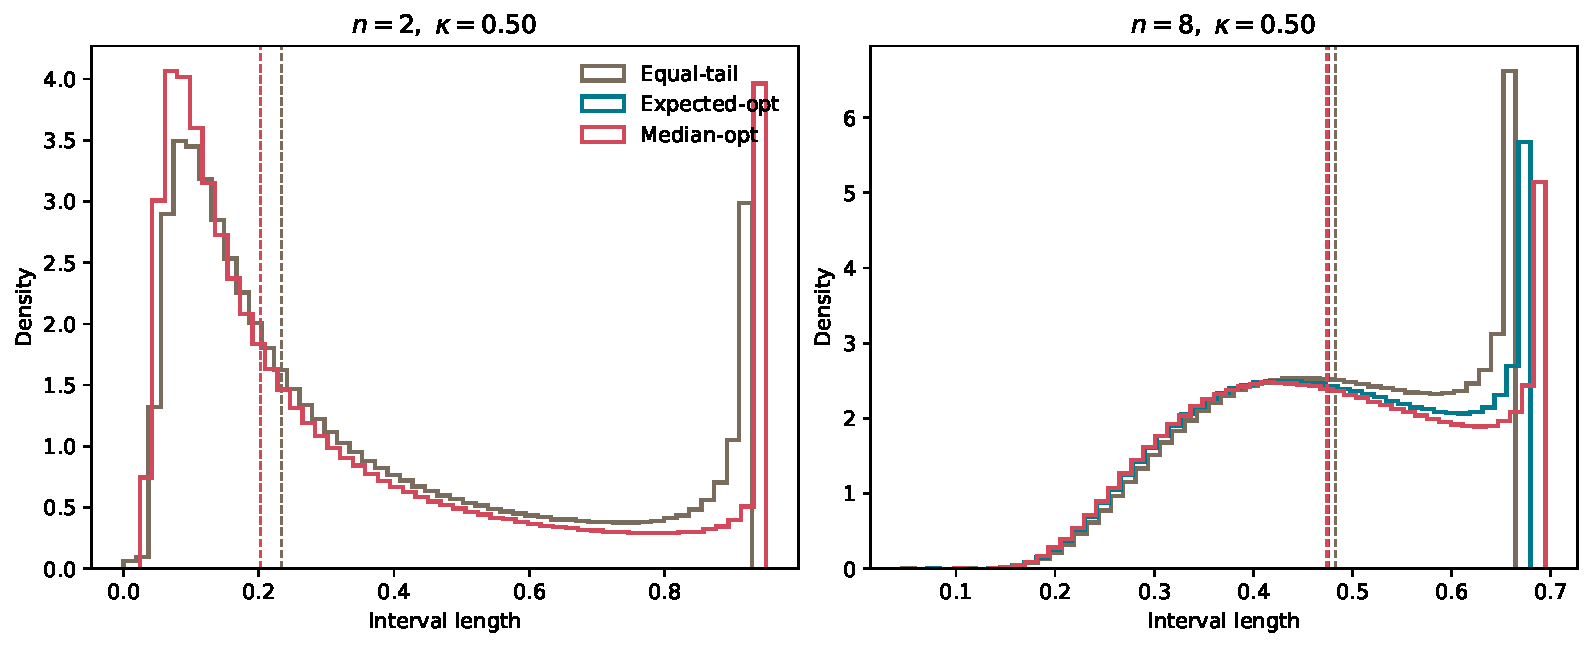
\includegraphics[width=\textwidth]{length_distribution.pdf}
\caption{Empirical distributions of interval length over the $\chi^2$ pivot for two representative settings. Dashed vertical lines mark the medians.}
\label{fig:lengths}
\end{figure}

Figure~\ref{fig:heatmaps} summarizes the full grid. The left panel visualizes how far the mean-to-median ratio can move from one; the right panel shows the median-length gain of the median-length interval over the expected-length interval. The first panel motivates the median criterion, while the second shows that the expected-length solution is already close to the median solution in most configurations considered here.

\begin{figure}[htbp]
\centering
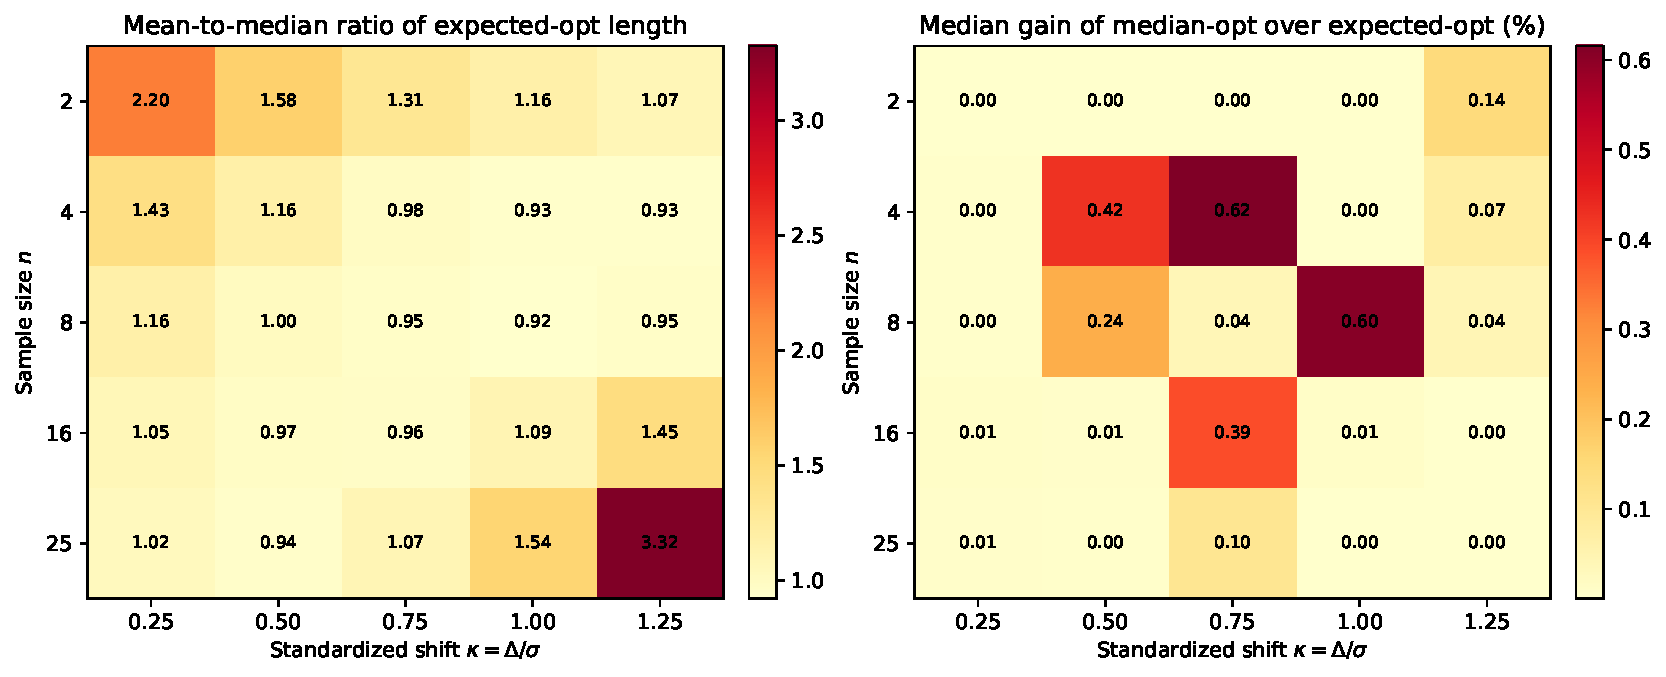
\includegraphics[width=\textwidth]{heatmaps.pdf}
\caption{Grid summaries for the expected-optimal and median-optimal intervals.}
\label{fig:heatmaps}
\end{figure}

\subsection{Monte Carlo sensitivity analysis}
Because the manuscript includes a Monte Carlo approximation to the median objective, it is helpful to quantify how much that approximation moves when the Monte Carlo size or seed changes. Table~\ref{tab:mcsens} reports four representative settings, varying the approximation over $R\in\{1000,4000,16000\}$ and including an alternate seed at $R=4000$. For each case, the table records the deterministic benchmark $p_M$, the Monte Carlo approximation $p_{MC}$, and the percentage change in the induced median interval length relative to the deterministic median-optimal interval.

Across the displayed settings, the substantive conclusions are stable. The largest deviation in the allocation itself is $|p_{MC}-p_M|=0.0014$, attained at $(n,\kappa)=(4,0.75)$ under $R=1000$, while the induced median length remains within $0.14\%$ of the deterministic benchmark throughout. In other words, the Monte Carlo approximation can move the reported optimizer slightly, especially in flatter parts of the objective, without changing the practical comparison of interval widths. This is consistent with treating the simulation-based version as a diagnostic companion to the deterministic computation rather than as a separate methodological contribution.

\begin{table}[htbp]
\centering
\caption{Sensitivity of the Monte Carlo median-length approximation to the simulation size $R$ and random seed in four representative settings. The column $\Delta \widetilde{m}$ reports the percentage change in median interval length relative to the deterministic median-optimal interval.}
\label{tab:mcsens}
\resizebox{\textwidth}{!}{\begin{tabular}{cclrrrr}
\toprule
$n$ & $\kappa$ & Config & $p_M$ & $p_{MC}$ & $|p_{MC}-p_M|$ & $\Delta \widetilde{m}$ (\%) \\
\midrule
2 & 0.50 & $R=1000$ & 0.0000 & 0.0001 & 0.0001 & 0.03 \\
2 & 0.50 & $R=4000$ & 0.0000 & 0.0001 & 0.0001 & 0.03 \\
2 & 0.50 & $R=4000$, alt. & 0.0000 & 0.0001 & 0.0001 & 0.03 \\
2 & 0.50 & $R=16000$ & 0.0000 & 0.0001 & 0.0001 & 0.05 \\
\midrule
4 & 0.75 & $R=1000$ & 0.0066 & 0.0052 & 0.0014 & 0.04 \\
4 & 0.75 & $R=4000$ & 0.0066 & 0.0062 & 0.0004 & 0.01 \\
4 & 0.75 & $R=4000$, alt. & 0.0066 & 0.0056 & 0.0009 & 0.02 \\
4 & 0.75 & $R=16000$ & 0.0066 & 0.0054 & 0.0011 & 0.02 \\
\midrule
8 & 1.00 & $R=1000$ & 0.0500 & 0.0499 & 0.0001 & 0.01 \\
8 & 1.00 & $R=4000$ & 0.0500 & 0.0499 & 0.0001 & 0.01 \\
8 & 1.00 & $R=4000$, alt. & 0.0500 & 0.0499 & 0.0001 & 0.01 \\
8 & 1.00 & $R=16000$ & 0.0500 & 0.0499 & 0.0001 & 0.01 \\
\midrule
25 & 1.25 & $R=1000$ & 0.0500 & 0.0499 & 0.0001 & 0.14 \\
25 & 1.25 & $R=4000$ & 0.0500 & 0.0499 & 0.0001 & 0.14 \\
25 & 1.25 & $R=4000$, alt. & 0.0500 & 0.0499 & 0.0001 & 0.14 \\
25 & 1.25 & $R=16000$ & 0.0500 & 0.0499 & 0.0001 & 0.14 \\
\bottomrule
\end{tabular}
}
\end{table}

\subsection{Monte Carlo validation}
Although coverage is exact by Proposition~1, the implementation should still be checked numerically. The repository therefore evaluates all $25$ design points in the $(n,\kappa)$ grid using $100{,}000$ Monte Carlo chi-squared draws per point. Because the coverage claim rests on the analytical proof rather than on simulation, the Monte Carlo exercise functions as a software check of the numerical integration and optimization routines rather than as empirical validation of the theorem itself. Across the full validation grid and all four methods, the estimated coverages range from $0.9492$ to $0.9514$, in line with the theoretical target of $0.95$. Table~\ref{tab:mc} reports four representative settings: a small-sample benchmark, the point of largest additional gain over the expected-length interval, a moderate-sample case where the median-length allocation shifts toward the upper boundary, and the high-power regime with the largest improvement over equal-tail intervals. Rows labeled ``Median-MC'' correspond to the simulation-based approximation. Only the estimated coverages and resulting interval lengths are shown, since those are the quantities of substantive interest.

\begin{table}[htbp]
\centering
\caption{Representative Monte Carlo validation settings drawn from the full $(n,\kappa)$ grid, based on $100{,}000$ chi-squared draws per setting.}
\label{tab:mc}
\resizebox{0.9\textwidth}{!}{\begin{tabular}{cccrrr}
\toprule
$n$ & $\kappa$ & Method & $\widehat{\Pr}\{\text{cover}\}$ & Mean length & Median length \\
\midrule
2 & 0.50 & Equal-tail & 0.9498 & 0.3415 & 0.2329 \\
2 & 0.50 & Expected-opt & 0.9503 & 0.3211 & 0.2024 \\
2 & 0.50 & Median-opt & 0.9503 & 0.3211 & 0.2024 \\
2 & 0.50 & Median-MC & 0.9503 & 0.3211 & 0.2025 \\
\midrule
4 & 0.75 & Equal-tail & 0.9499 & 0.5958 & 0.6195 \\
4 & 0.75 & Expected-opt & 0.9497 & 0.5899 & 0.6037 \\
4 & 0.75 & Median-opt & 0.9496 & 0.5928 & 0.6002 \\
4 & 0.75 & Median-MC & 0.9496 & 0.5932 & 0.6002 \\
\midrule
8 & 1.00 & Equal-tail & 0.9499 & 0.5590 & 0.6103 \\
8 & 1.00 & Expected-opt & 0.9514 & 0.5187 & 0.5633 \\
8 & 1.00 & Median-opt & 0.9513 & 0.5248 & 0.5599 \\
8 & 1.00 & Median-MC & 0.9512 & 0.5225 & 0.5600 \\
\midrule
25 & 1.25 & Equal-tail & 0.9496 & 0.0071 & 0.0027 \\
25 & 1.25 & Expected-opt & 0.9493 & 0.0041 & 0.0012 \\
25 & 1.25 & Median-opt & 0.9493 & 0.0041 & 0.0012 \\
25 & 1.25 & Median-MC & 0.9492 & 0.0041 & 0.0012 \\
\bottomrule
\end{tabular}
}
\end{table}

\section{Discussion}
The median-length interval studied here is a coherent extension of the exact-coverage expected-length interval of \citet{chakraborti2012shortest}. Its main value is interpretive rather than dramatic numerical superiority: it targets the typical realized interval width, which can differ materially from the mean width in finite samples. On the numerical grid studied here, the median-length interval modestly improves the median width relative to the expected-length interval and can substantially improve on equal-tail intervals. That combination of findings is not contradictory. Rather, it shows that a meaningful distinction between average and typical width can coexist with near-optimality of the expected-length rule under the alternative median criterion. The added Monte Carlo approximation reinforces that conclusion rather than changing it: once the pivot reduction is exploited, a deterministic grid already captures the relevant one-dimensional distribution with high stability, and the simulation-based version mainly serves as a robustness check and as a bridge to practitioners who prefer simulation-based workflows.

The results also suggest a practical recommendation. If the design objective is explicitly average loss, the expected-length interval remains a reasonable default. If the practitioner cares more about the width they are likely to see in a typical realization, the median-length interval provides an exact-coverage alternative with essentially the same computational burden. When a simulation-based implementation is operationally more natural, the Monte Carlo version offers a close approximation to the deterministic computation without changing the underlying coverage argument. In that sense, the median criterion is best viewed as a calibrated companion to the expected-length benchmark rather than a universal replacement for it.

The simulation-based approximation should not, however, be over-interpreted. Its reported optimizer depends on the Monte Carlo size $R$, on the fixed common-random-numbers sample used to stabilize comparisons across candidate $p$ values, and on the nonsmooth sample-median objective. In flat parts of the objective, or near the admissible boundaries, modest changes in $R$ or in the simulated sample can shift the reported optimizer while leaving the achieved interval lengths nearly unchanged. The present calculations with $R=4{,}000$ are therefore best understood as demonstrating numerical stability of the substantive conclusions, not as establishing a separate asymptotic theory for the Monte Carlo optimizer.

Several extensions remain open. The present note treats only the one-sample upper-tailed t-test and fixed $(\alpha,\gamma)=(0.05,0.05)$. It would be natural to revisit two-sided tests, two-sample t procedures, or other robust summaries of random interval width. It would also be useful to complement the present numerical optimization with theory on uniqueness, boundary behavior, or convergence of the median-length allocation as the design grid is refined.

The method developed here should also be understood within the context of recent debates about the role of power in statistical practice. Work by \citet{ginersorolla2024power} emphasizes that power analysis is meaningful only relative to a defensible target effect, while \citet{riesthuis2024power} shows how confidence-interval ideas can be embedded in prospective simulation workflows for minimum-effect and equivalence testing. More broadly, \citet{irmer2024mspe} develops model-implied simulation-based power estimation for settings far beyond the simple t-test. These approaches address design-stage questions that are conceptually distinct from the object studied here, but they also clarify its role. The present method is indexed by a prespecified standardized alternative and its exact-coverage claim is pointwise in that index; it is not a replacement for prospective power planning or for post-data effect estimation. Its more modest role is to provide an exact low-dimensional finite-sample benchmark for how power intervals behave once a standardized target has already been fixed, thereby complementing modern simulation-based and design-oriented workflows rather than competing with them.

\bibliographystyle{plainnat}
\bibliography{paper}

\end{document}
